%!TEX root=../../main.tex
\section{Frontend}
In diesem Kapitel wird die Erstellung eines Konzepts für das Frontend erläutert. Dabei müssen Faktoren wie beispielsweise unsere Zielgruppe, die Lehrerschaft beachtet werden. Im folgenden Kapitel werden die theoretischen Hintergründe des Konzeptes überlegt, danach werden erste Entwürfe mittels Mockups erstellt. 
\subsection{Vorbereitung}
Wie im Kapitel 5.1 und 5.3 festgelegt wird im Frontend Bootstrap in Verbindung mit VueJS verwendet. Zu aller Erst muss daher VueJS auf dem Computer, auf dem das Projekt erstellt wir installiert werden. Dies geschieht auf Windows über den Node Packet Manager (NPM) \cite{vue-install}. Der Befehl um VueJS zu installieren schaut wie folgt aus:
\begin{code}{bash}
	npm install -g @vue/cli
\end{code}
Nachdem VueJS installiert ist kann man in das gewünschte Verzeichnis wechseln und über
\begin{code}{bash}
	vue create refundable
\end{code}
ein neues Vue Projekt erstellen, das in diesem Fall \enquote{Refundable} heißt \cite{vue-create-project}. Um die Funktionalität von Bootstrap und VueJS optimal auszunutzen wird Bootstrap direkt mit dem Node Packet Manager zu VueJS installiert \cite{bootstrap-vue-getting-started}:
\begin{code}{bash}
	npm install vue bootstrap-vue
\end{code}
Damit ist die Arbeit aber noch nicht getan, um in den Komponenten Bootstrap und dessen vordefinierte Icons zu verwenden, muss man in \enquote{main.js} folgendes importieren:
\begin{code}{html}
	import { BootstrapVue, BootstrapVueIcons } from "bootstrap-vue";
	import "./plugins/bootstrap-vue";
	
	Vue.use(BootstrapVue);
	Vue.use(BootstrapVueIcons);
\end{code}
\captionof{listing}{Benötigte Befehle um Bootstrap im VueJS Projekt einzubinden}
	\label{list:requcommands} ~\\
Alle Teile der Website sind in sogenannten Komponenten verpackt, die je nach Benutzereingaben dynamisch gewechselt werden. 

\newpage
\subsection{Komponenten der Website}
\subsubsection{Generell}
Die Struktur der Komponenten ist so aufgebaut, dass die Seite sowohl für Desktop- als auch mobile Endgeräte optimiert ist. Dazu wird das \enquote{Grid-System} von Bootstrap verwendet, welches seinen Platz im \enquote{template-Tag}, der VueJS Komponente findet. Dieses besteht aus einem Container, einer Reihe (Row) und einer Spalte (Column). Da es am Anfang das Problem gab, dass nicht der ganze Bildschirm ausgenutzt wird, habe ich folgende Klassen in unserem CSS-Dokument erstellt:
\begin{code}{css}
	.template-main-container {
		height: 100vh;
		width: 100vw;
		margin: 0;
		padding: 0;
	}
	
	.template-main-row {
		height: 100vh;
		width: 100vw;
		margin: 0;
		padding: 0;
	}
\end{code}
\captionof{listing}{CSS Klassen für die Haupt- Contianer und Reihen}
	\label{list:cssmaincont} ~\\
Diese dienen dazu, dass der Hauptcontainer, als auch die Hauptreihe der Website, 100\% der Höhe (100 vertikale Einheiten), sowie 100\% der Breite (100 horizontale Einheiten) einnehmen. Außerdem wird in den Klassen definiert, dass die Elemente keinen Abstand zum Rand haben sollen.
\newpage
\subsubsection{Login-Seite}
Uns war sehr wichtig, dass die Login-Seite sehr schlicht gehalten ist und sofort zu verstehen ist. Da das Tool Refundable nur von Lehrern des TGMs verwendet werden soll, haben wir uns dazu entschlossen, dass in der Loginmaske die E-Mail-Endung \enquote{@tgm.ac.at} vordefiniert und unveränderbar ist. Außerdem wollten wir dem Aufrufer der Website sofort klar machen, um was es sich bei dieser Website handelt und haben daher den Projektnamen Refundable, als auch unseren Slogan auf der Seite platziert. Des weiteren war aufgrund der DSGVO eine Meldung zu realisieren, die den Benutzer darüber informiert, dass Cookies verwendet werden. Falls diese Meldung nicht akzeptiert wird und man versucht sich anzumelden, wird eine Fehlermeldung dargestellt. Diese Meldung wird jedoch dynamisch mit VueJS erstellt und nicht direkt mittels Bootstrap. In der Realität schaut die Login-Seite wie folgt aus (Abbildung 7.1):
\begin{figure}[H]
	\centering
	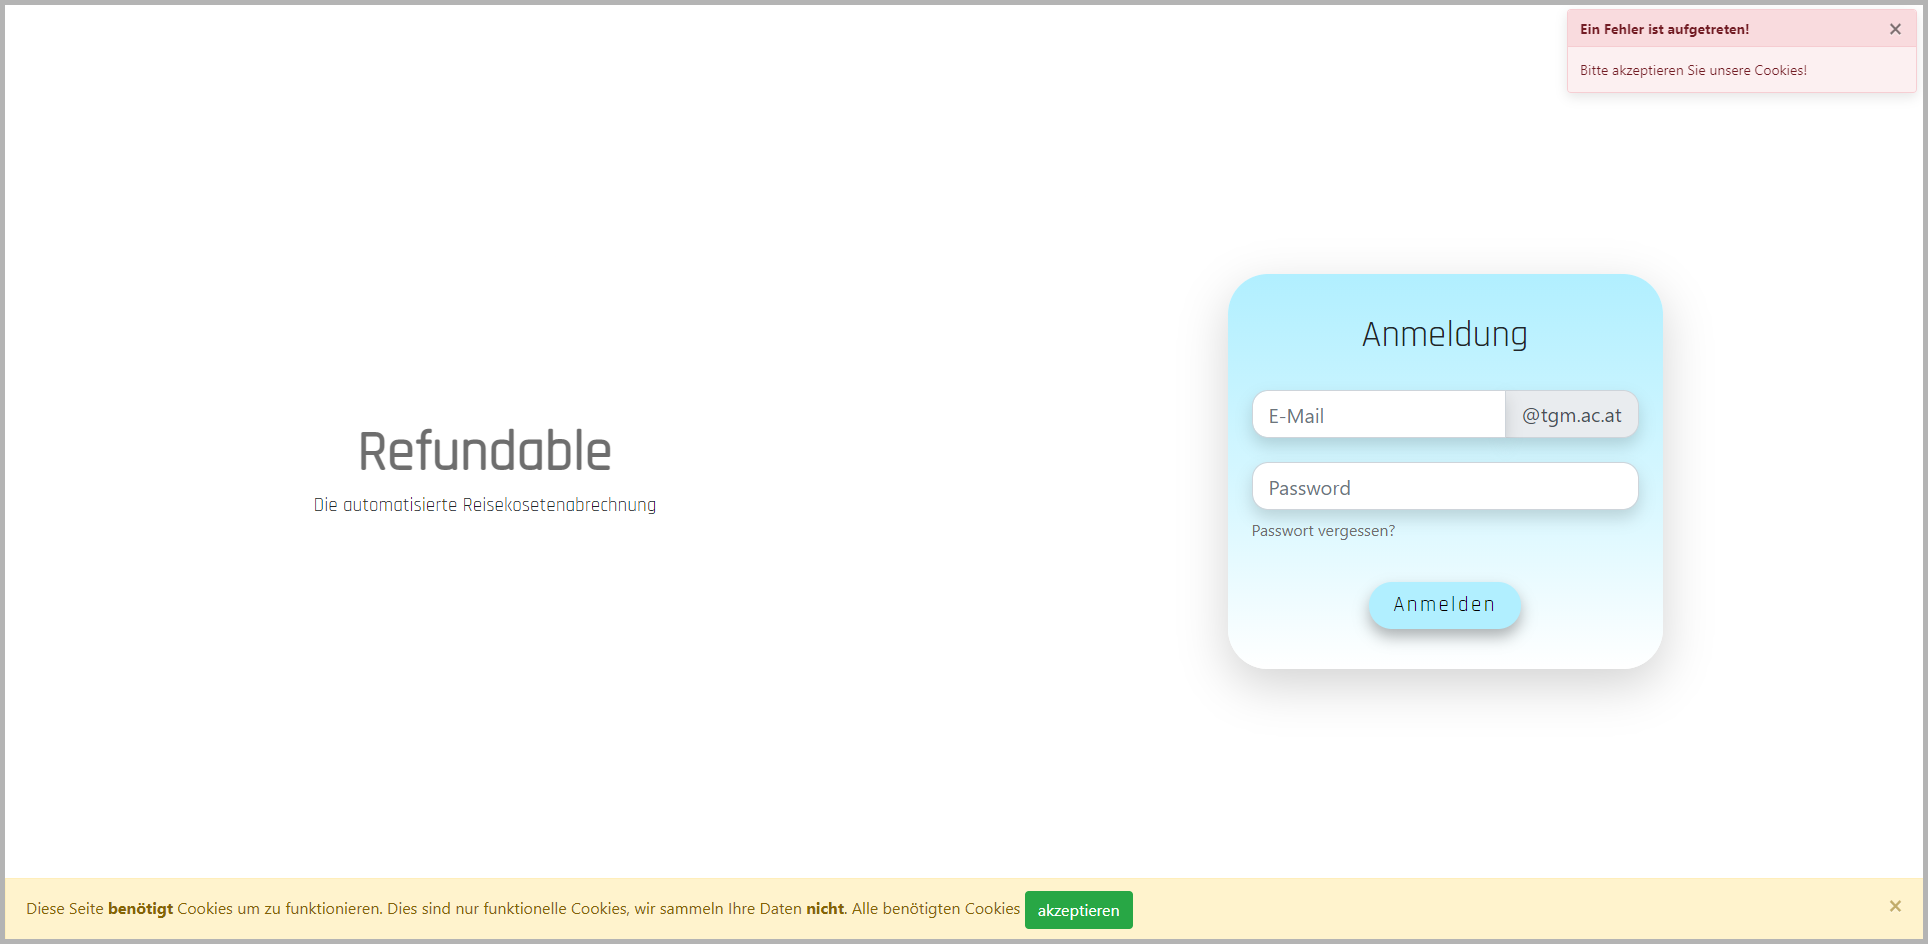
\includegraphics[width=1\linewidth]{images/website/login}
	\caption[Login]{Ein Bild der endgültigen Login-Seite}
	\label{fig:login}
\end{figure}
\paragraph{Login-Maske}
~\\
Die Login-Maske besteht aus einem eigenen Container, welcher ermöglicht die Maske vollkommen responsiv aufzubauen. Die Eingabefelder haben wir mit einer \enquote{input-groupe} gelößt (Code Z. 12). Um einen Wert optisch in einem Eingabefeld vorzugeben hat Bootstrap ein praktisches Element, namens \enquote{b-input-groupe-text} (Code Z. 14), welches vor oder nach dem Feld hinzugefügt werden kann. Da die Login-Daten, der TGM Server verwendet werden, haben wir einen Link eingebaut, falls man sein Passwort vergessen hat. Betätigt man diesen, wird man auf die entsprechende Seite des TGMs weitergeleitet.
\begin{code}{html}
	<!-- Anmeldungsformular -->
	<b-col cols="12" md="6">
		<b-container>
			<b-row align-h="center">
				<b-col cols="12" sm="10" md="10" lg="8" xl="6">
					<b-container id="login-wrap" class="shadow-lg">
						<b-row id="r-login" align-h="center">
							<h2 id="lheading2">Anmeldung</h2>
						</b-row>
						<b-row align-h="center" id="r-email">
							<b-col cols="12">
								<!-- Input des Benutzernamens / der Email -->
								<b-input-group size="lg">
									<b-input-group-text
										id="tgm-addon"
										class="shadow"
										slot="append"
										><span>@tgm.ac.at</span></b-input-group-text
										>
									<b-form-input
										id="email"
										class="shadow login-inputs"
										v-model="email"
										type="text"
										placeholder="E-Mail"
									></b-form-input>
								</b-input-group>
							</b-col>
						</b-row>
						<b-row id="r-password">
							<b-col cols="12">
								<!-- Input des Passworts -->
								<b-form-input
									id="password"
									class="shadow login-inputs"
									v-model="password"
									type="password"
									placeholder="Password"
									size="lg"
								></b-form-input>
							</b-col>
						</b-row>
						<b-row id="r-forgotten">
							<b-col cols="12">
								<!-- Passwort vergessen Weiterleitung auf Moodle -->
								<a
									id="forgotten-password"
									href="https://elearning.tgm.ac.at/login/forgot_password.php"
								>Passwort vergessen?</a
								>
							</b-col>
						</b-row>
						<b-row align-h="center" id="r-login-btn">
							<!-- Login Button -->
							<b-button size="lg" id="login-btn" v-on:click="login"
							>Anmelden</b-button
							>
						</b-row>
					</b-container>
				</b-col>
			</b-row>
		</b-container>
	</b-col>
\end{code}
\captionof{listing}{HTML Code der Login-Maske}
	\label{list:loginmask} ~\\
Da einige Elemente unseren Ansprüchen optisch nicht genügt haben, haben wir eigene Änderungen in unserem CSS-Code hinzugefügt. Dabei wurde vor allem die Gestaltung, der Eingabefelder und des Buttons verändert, aber auch die des Containers, welcher die Maske beinhaltet. Genauer gesagt haben wir den Farbverlauf des Logos in der Maske eingebaut, die Ecken der Elemente etwas abgerundet und Schatten hinzugefügt.
\begin{code}{css}
/* -- Login -- */

#login-wrap {
	background: rgb(255, 255, 255);
	background: -moz-linear-gradient(
	0deg,
	rgba(255, 255, 255, 1) 0%,
	rgba(220, 248, 255, 1) 38%,
	rgba(177, 239, 255, 1) 100%
	);
	background: -webkit-linear-gradient(
	0deg,
	rgba(255, 255, 255, 1) 0%,
	rgba(220, 248, 255, 1) 38%,
	rgba(177, 239, 255, 1) 100%
	);
	background: linear-gradient(
	0deg,
	rgba(255, 255, 255, 1) 0%,
	rgba(220, 248, 255, 1) 38%,
	rgba(177, 239, 255, 1) 100%
	);
	filter: progid: DXImageTransform.Microsoft.gradient(startColorstr="#ffffff", endColorstr="#b1efff", GradientType=1);
	padding: 1.5rem;
	border-radius: 2.5rem;
}

#email {
	border-radius: 1rem 0 0 1rem;
}

#tgm-addon {
	border-radius: 0 1rem 1rem 0;
}

.input-group-append {
	border-radius: 0 1rem 1rem 0;
}

.input-group-text {
	border-radius: 0 1rem 1rem 0;
}

#password {
	border-radius: 1rem 1rem 1rem 1rem;
}

#login-btn {
	font-family: "Rajdhani", sans-serif;
	padding: 0.5rem 1.5rem 0.5rem 1.5rem;
	font-size: 1.3rem;
	letter-spacing: 2.5px;
	font-weight: 500;
	color: #000;
	background-color: rgba(177, 239, 255, 1);
	border: none;
	border-radius: 45px;
	box-shadow: 0px 8px 15px rgba(0, 0, 0, 0.3);
	transition: all 0.3s ease 0s;
	cursor: pointer;
	outline: none;
}

#login-btn:hover {
	background-color: #2ec0e5;
	box-shadow: 0px 15px 20px rgba(46, 229, 157, 0);
	color: #fff;
	transform: translateY(3px);
}
\end{code}
\captionof{listing}{CSS Code der Login-Maske}
	\label{list:csslogin} ~\\
\paragraph{Cookie-Meldung}
~\\
Die Meldung, dass Cookies benutzt werden, sollte schlicht und einfach sein. Außerdem haben wir uns als Ziel gesetzt, dass sie dem Nutzer deutlich klar machen soll, dass wir ausschließlich funktionelle und notwendige Cookies verwenden. Für diese Meldung hat sich perfekt das vordefinierte \enquote{Alert-Element} von Bootstrap geeignet:
\begin{code}{html}
	<!-- Bestätigung, dass diese Seite Cookies benutzt -->
	<b-alert
		v-model="showBottom"
		class="position-fixed fixed-bottom m-0 rounded-0"
		style="z-index: 2000;"
		variant="warning"
		dismissible
	>
		Diese Seite <b>benötigt</b> Cookies um zu funktionieren. Dies sind nur
		funktionelle Cookies, wir sammeln Ihre Daten <b>nicht</b>. Alle benötigten
		Cookies
		<!-- Button zum akzeptieren -->
		<b-button variant="success" @click="validateCookies()"
			>akzeptieren
		</b-button>
	</b-alert>
\end{code}
\captionof{listing}{HTML Code Cookie akzeptieren }
	\label{list:cookiehtml} ~\\
\newpage
\subsubsection{Startseite}
Die Startseite sollte so intuitiv und übersichtlich wie möglich sein. Deswegen haben wir uns für ein \enquote{Drei Spalten Design} entschieden. In der ersten Spalte befinden sich alle wichtigen Funktionen - drei Knöpfe, zum erstellen von neuen Anträgen, um alle aktiven Anträge anzuschauen und um alle Anträge zu betrachten, die man jemals gestellt hat. In der 2. Spalte befindet sich das Logo, eine Illustration für das Dashboard und ein Knopf zum Ausloggen. Falls man ein Administrator ist, wird hier ebenfalls ein Knopf, zum wechseln in die Administratoransicht angezeigt. In der dritten Spalte werden Neuigkeiten zu den Anträgen des Benutzers angezeigt, falls man auf eine Neuigkeit klickt, wird man zu dem jeweiligen Antrag weitergeleitet. In der Realität schaut die Startseite wie folgt aus (Abbildung 7.2):
\begin{figure}[H]
	\centering
	
\includegraphics[width=1\linewidth]{images/website/dashboard}
	\caption[Dashboard]{Ein Bild der endgültigen Startseite}
	\label{fig:dashboard}
\end{figure}
Jedoch ist dieses System auf mobilen Geräten nicht sonderlich übersichtlich, deshalb haben wir diese etwas abgeändert. Diese ist sehr schlicht gehalten, jedoch macht dies das Ganze auf Smartphones um einiges einfacher die Website zu bedienen. Die mobile Version der Startseite schaut in der Realität wie folgt aus (Abbildung 7.3):
\begin{figure}[H]
	\centering
	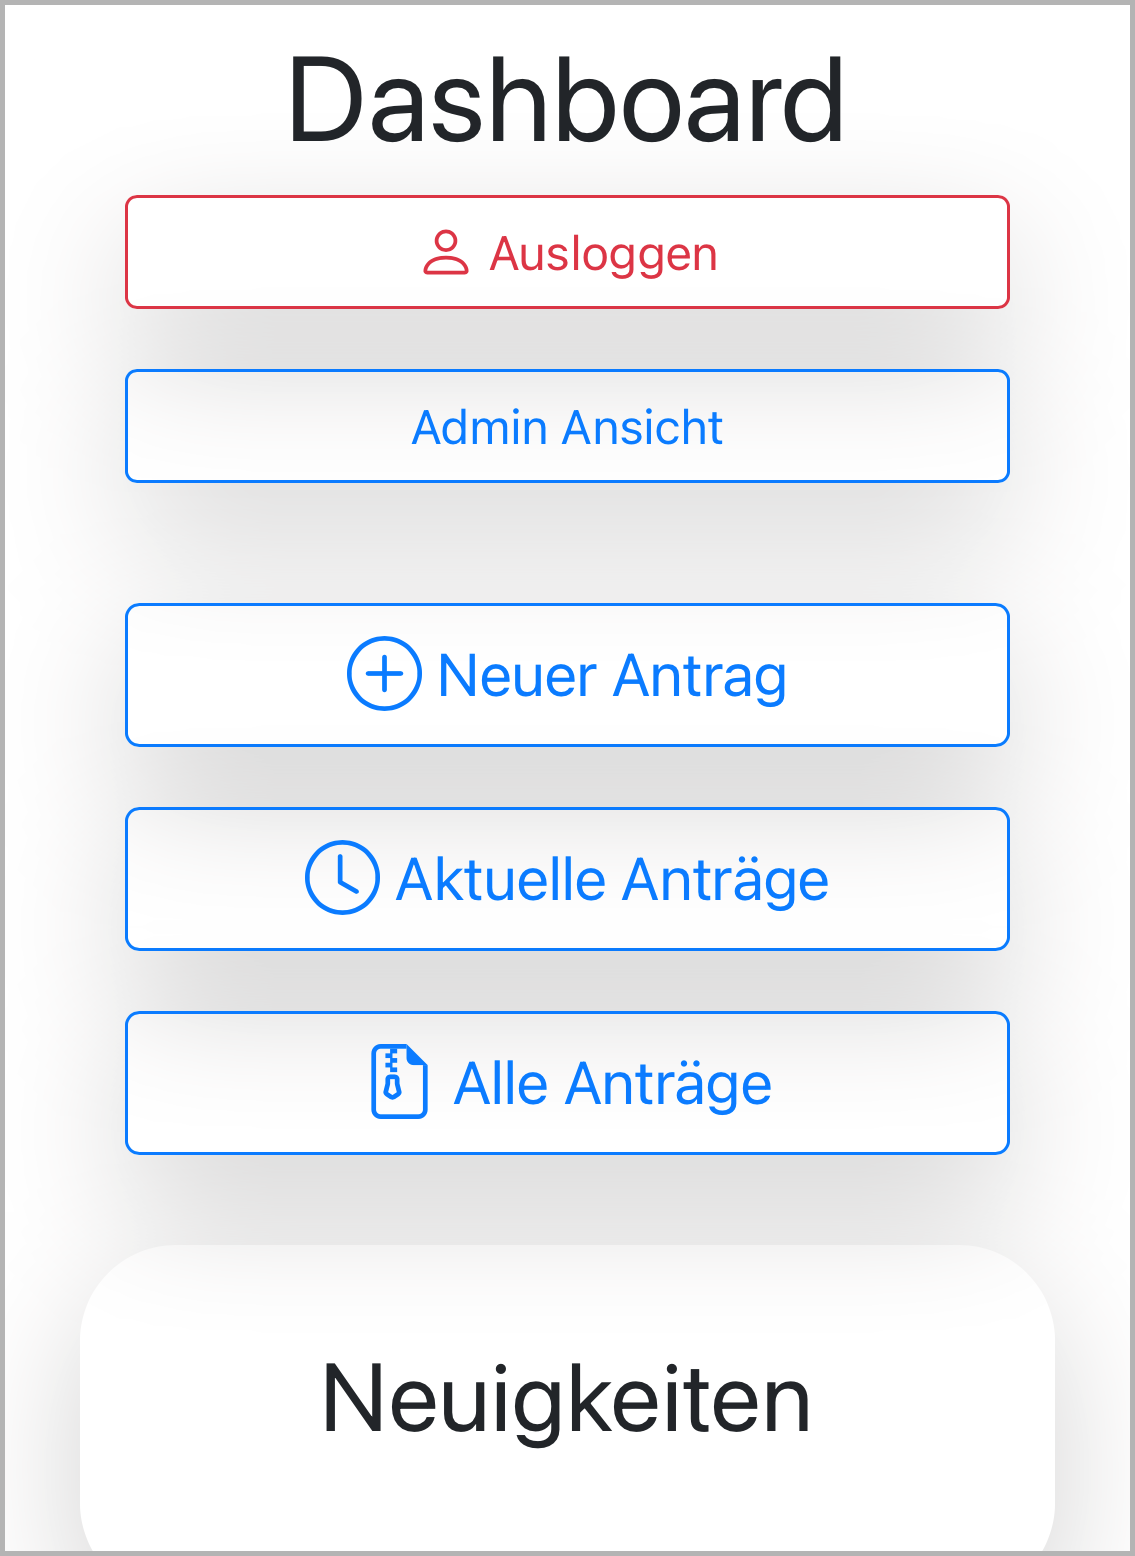
\includegraphics[width=0.4\linewidth]{images/website/dashboard_mobile}
	\caption[Dashboard Mobil]{Ein Bild der endgültigen Startseite (Mobil)}
	\label{fig:dashboardmobile}
\end{figure}

\paragraph{Menü-Element Desktop}
~\\
Der Container mit den Funktionselementen, hat wie beim Login einen Schatten, der ihn von dem Hintergrund abhebt. In diesem Container befinden sich die Menü Bezeichnung und die klickbaren Elemente, die auch aus einem Container bestehen und eine responsive Illustration, die zu der jeweiligen Funktion passt und eine Bezeichnung, was dieser Knopf auslöst beinhaltet.
\begin{code}{html}
<b-col id="dash-main-cont" class="d-none d-md-block" cols="12" md="4">
	<b-container>
		<b-row
			id="dash-row"
			align-v="center"
			align-h="center"
			class="shadow-xl"
		>
			<b-col cols="12">
				<center><h2 id="menu-h2">Menü</h2></center>
			</b-col>
			<!-- Custom Button für einen neuen Antrag -->
			<b-col
				id="new"
				cols="12"
				class="shadow-lg dash-elem"
				v-on:click="newApplication"
			>
				<b-container style="height: 100%">
					<b-row align-h="center" align-v="center" style="height: 100%">
						<b-col cols="6" class="ill-wrapper d-none d-md-block">
						<!-- Illustration neuer Antrag -->
							<b-img
								id="all-ill"
								center
								src="@/assets/new.svg"
								alt="Illustration für alle Anträge"
							></b-img>
						</b-col>
						<b-col cols="12" md="6">
							<h2 id="new-h2" class="dh">Neuer Antrag</h2>
						</b-col>
					</b-row>
				</b-container>
			</b-col>
			
			...
		</b-row>
	</b-container>
</b-col>
\end{code}
\captionof{listing}{HTML-Code-Teile des Startseitenmenüs}
	\label{list:menuhtml} ~\\
Optisch wurde vor allem die Höhe des umschließenden Containers verändert, und dessen umliegende Abstände. Wie man auf der Abbildung 7.2 sehen kann wurden hier auch wieder die Ecken abgerundet. Was man jedoch nicht sehen kann, ist, dass sich die Funktionselemente, optisch absenken und der Schatten entfernt wird und die Farbe verändert wird, wenn man mit der Maus, die sich zu einer zeigenden Hand verändert, über das Element fährt. 
\begin{code}{css}
#dash-main-cont {
	height: 70vh;
}

#dash-row {
	height: 70vh;
	padding-left: 2rem;
	padding-right: 2rem;
	padding-bottom: 1.5rem;
}

.dash-elem {
	background-color: rgb(255, 255, 255);
	height: 22%;
	transition: all 0.3s ease 0s;
	cursor: pointer;
	outline: none;
}

.dash-elem:hover {
	background-color: #8ff2ff;
	box-shadow: 0px 0px 50px rgba(0, 0, 0, 0.144);
	color: rgb(141, 141, 141);
	transform: translateY(3px);
}

#dash-row {
	border-radius: 6rem 6rem 6rem 6rem;
}
\end{code}
\captionof{listing}{Teile des CSS Codes, des Startseitenmenüs}
	\label{list:cssmenu} ~\\
\paragraph{Menü-Element Mobil}
~\\
Wie schon erwähnt ist die mobile Ansicht sehr schlicht gehalten, damit sie nicht überladen wirkt und dass sich auch vor allem die nicht Technik affinen Lehrer auskennen. Daher zeigen wir auf der mobilen Ansicht nur das Nötigste an (Siehe Abbildung 7.3). Alle Knöpfe werden nun vertikal angeordnet und mit einem passenden Icon bestückt. Die Newselemente unterscheiden sich kaum von denen, der Desktop-Version, die Elemente sind lediglich mit etwas weniger Details bestückt und sind nicht in einem scrollbaren Container, da man auf der mobilen Version sonst doppelt scrollen müsste.
\begin{code}{html}
	<!-- DASH MOBILE -->
	<b-col class="d-block d-md-none" cols="12">
	  <!-- Column -->
	  <b-container fluid>
		<b-row align-v="center" align-h="center">
		  <b-col cols="12">
			<center><h1 style="margin-top:10px;">Dashboard</h1></center>
		  </b-col>
		  <b-col cols="12">
			<!-- Logout Button -->
			<b-button
			  variant="outline-danger"
			  class="shadow-lg"
			  v-on:click="logout"
			  style="margin-top:0px; margin-bottom:20px; width:100%"
			>
			  <b-icon icon="person" aria-hidden="true"></b-icon> Ausloggen
			  <!-- Icon -->
			</b-button>
		  </b-col>
		  <b-col cols="12">
			<!-- Neuer Antrag Button --><b-button
			  size="lg"
			  variant="outline-primary"
			  v-on:click="newApplication"
			  class="shadow-lg"
			  style="margin-bottom:20px; width:100%"
			>
			  <b-icon icon="plus-circle" aria-hidden="true"></b-icon> Neuer
			  Antrag
			</b-button></b-col
		  >	
\end{code}
\captionof{listing}{Teile des HTML-Codes der mobilen Startseite}
	\label{list:startmobile} ~\\
\paragraph{Neuigkeiten-Element}
~\\
Die Neuigkeiten-Elemente sind mit einer Illustration bestückt, die den momentanen Status, des jeweiligen Antrags beschreiben soll. Außerdem wird ein Titel der Neuigkeit mitgegeben, die zum Beispiel \enquote{Antrag X abgelehnt} heißen könnte. Etwas mehr Details werden dann noch in einem Beschreibungsfeld mitgegeben, das wegen der Übersichtlichkeit nur auf Desktopgeräten sichtbar ist.
\begin{code}{html}
	<b-row align-v="center">
	<b-col cols="2">
	  <b-container style="height: 100%">
		<b-row align-v="center" align-h="center" style="height: 100%">
		  <!-- Illustration Angenommen/Abgelehnt -->
		  <img
			src="@/assets/accepted_1.svg"
			class="align-middle news-status"
			style="height: 50px; width: auto"
			alt="Illustration von arbeitenden Personen"
		  />
		</b-row>
	  </b-container>
	</b-col>
	<b-col cols="10">
	  <b-container>
		<b-row align-h="center" align-v="center">
		  <b-col cols="12">
			<!-- Titel der Neuigkeit -->
			<h3 class="news-elem-heading">{{ snews.title }}</h3>
		  </b-col>
		</b-row>
		<b-row align-h="center" class="d-none d-md-block">
		  <b-col cols="12">
			<!-- Beschreibung der Neuigkeit -->
			<h4 class="news-elem-heading">{{ snews.description }}</h4>
		  </b-col>
		</b-row>
	  </b-container>
	</b-col>
  </b-row>	
\end{code}
\captionof{listing}{HTML Code, des Neuigkeiten Elementes}
	\label{list:htmlnews} ~\\
\newpage
\subsubsection{Neuer Antrag}
Auf diese Seite gelangt der Nutzer entweder, durch die Betätigung des \enquote{Neuer Antrag} Buttons auf der Startseite, oder über die Verknüpfung auf der \enquote{Alle Anträge} oder \enquote{Aktive Anträge} Ansicht. Da es nicht möglich ist ein einheitliches Formular zu kreieren, haben wir uns dazu Entschieden, vor dem Formular eine Auswahlmöglichkeit der Antragsart einzubauen.
\paragraph{Auswahl}
~\\
Die von uns gewählte Auswahlmöglichkeit ist sehr einfach und intuitiv gestaltet. Die drei verschiedenen Hauptarten von Anträgen sind klar und deutlich zu unterscheiden. Optisch sind die Knöpfe ähnlich strukturiert, wie die der Hauptseite, damit sich ein einheitliches Design, durch die Website zieht.
\begin{figure}[H]
	\centering
	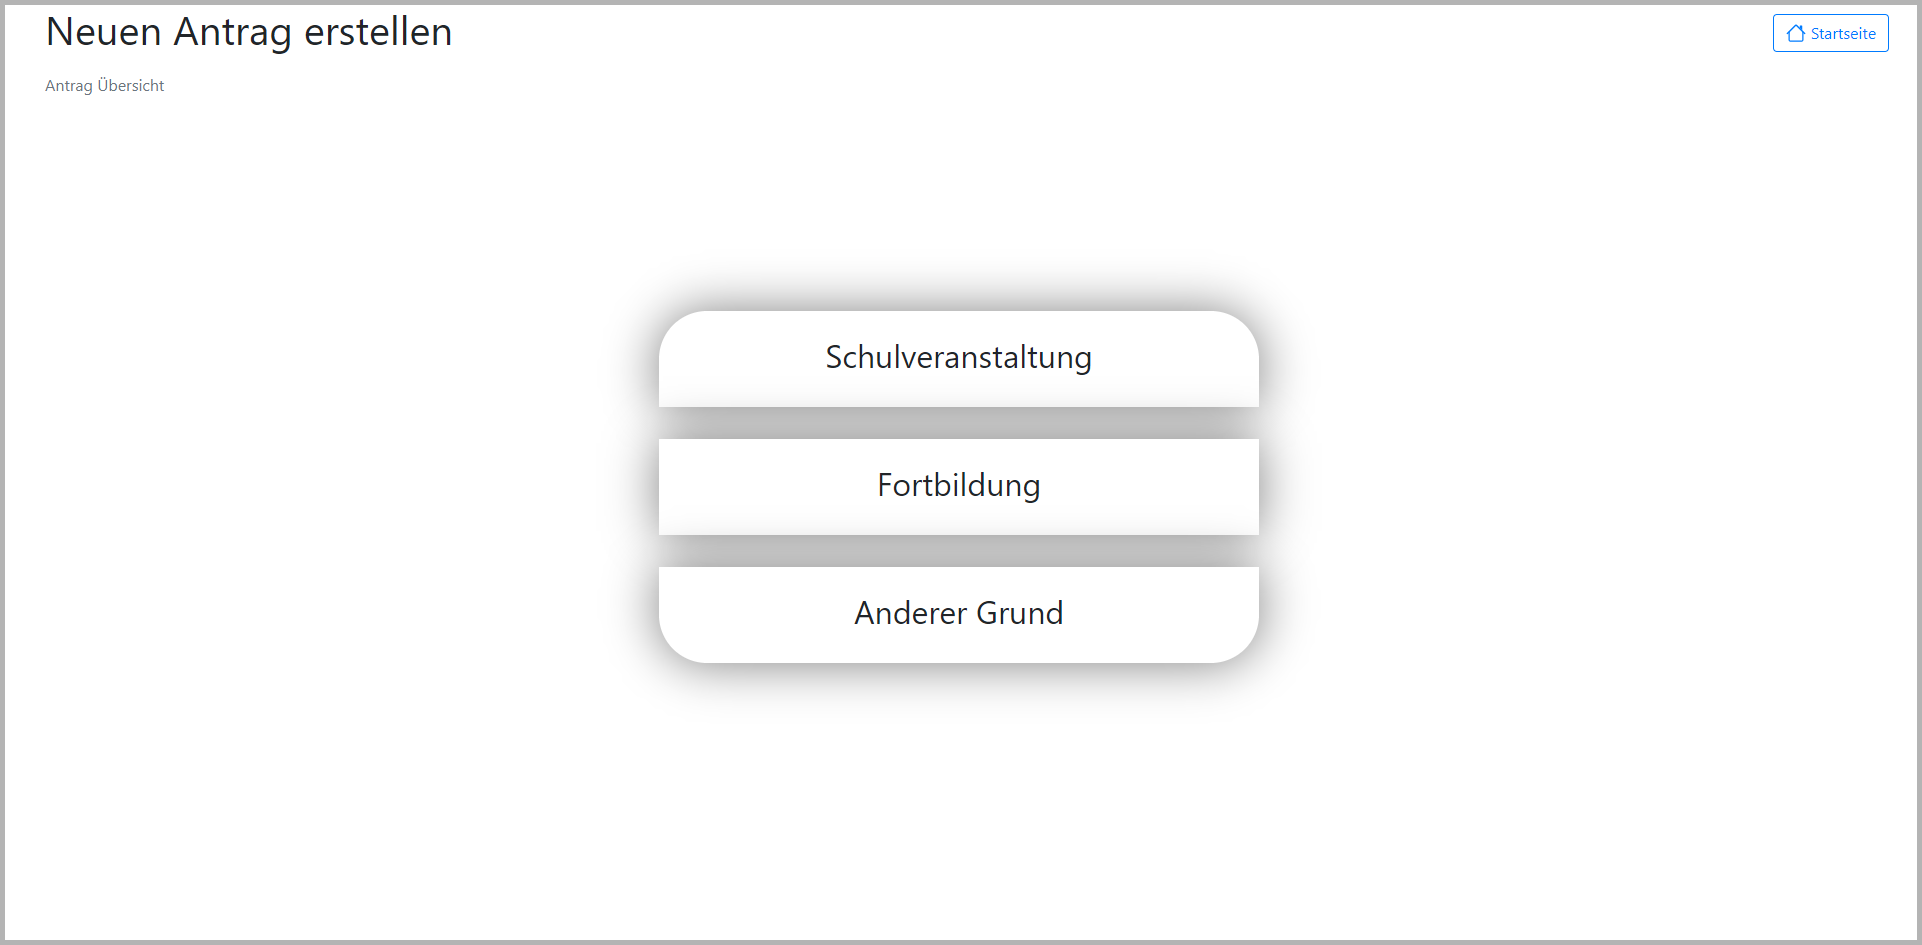
\includegraphics[width=1\linewidth]{images/website/neu}
	\caption[Neuer Antrag Auswahl]{Ein Bild der endgültigen Seite, um ein einen neuen Antrag auszuwählen}
	\label{fig:neuauswahl}
\end{figure}
Die Knöpfe sind wiedermals in eigenen Containern dargestellt, um sie optimal der Größe des Endgerätes anzupassen. In dem Container, der sich mit einem Schatten vom Hintergrund abhebt, ist eine eindeutige Bezeichnung, der Funktion, des jeweiligen Elementes. Fährt man mit der Maus über einen Knopf, wird dieser, wie auf der Startseite in seiner Farbe verändert.
\begin{code}{html}
	<b-container id="school-button" class="na-elem shadow-xl">
	<!-- Custom Button zum erstellen eines Schulantrages -->
	<b-row
	  class="na-elem-sr"
	  align-v="center"
	  v-on:click="school()"
	>
	  <b-col cols="12">
		<h2 class="na-elem-h">Schulveranstaltung</h2>
	  </b-col>
	</b-row>
  </b-container>	
\end{code}
\captionof{listing}{HTML Code, einer Auswahlmöglichkeit}
	\label{list:htmlselect} ~\\
\paragraph{Schulveranstaltung}
~\\
Der Antrag für eine neue Schulveranstaltung ist der komplexeste Antrag, mit den meisten Eingabefeldern. Außerdem gehören zu dem Antrag für eine Schulveranstaltung auch die Begleitpersonen Anträge. Um die Eingabe von Uhrzeiten und Daten einfacher zu machen, haben wir die Elemente \enquote{b-form-datepicker} und \enquote{b-form-timepicker} verwendet. Dies sind standardmäßige Elemente, die von BootstrapVue vordefiniert sind. Um den Lehrern auf den ersten Blick klar zu machen, welche Daten in welches Feld eingefügt werden, haben wir alle Eingabefelder mit einem Titel und einer Info bestückt.
\begin{figure}[H]
	\centering
	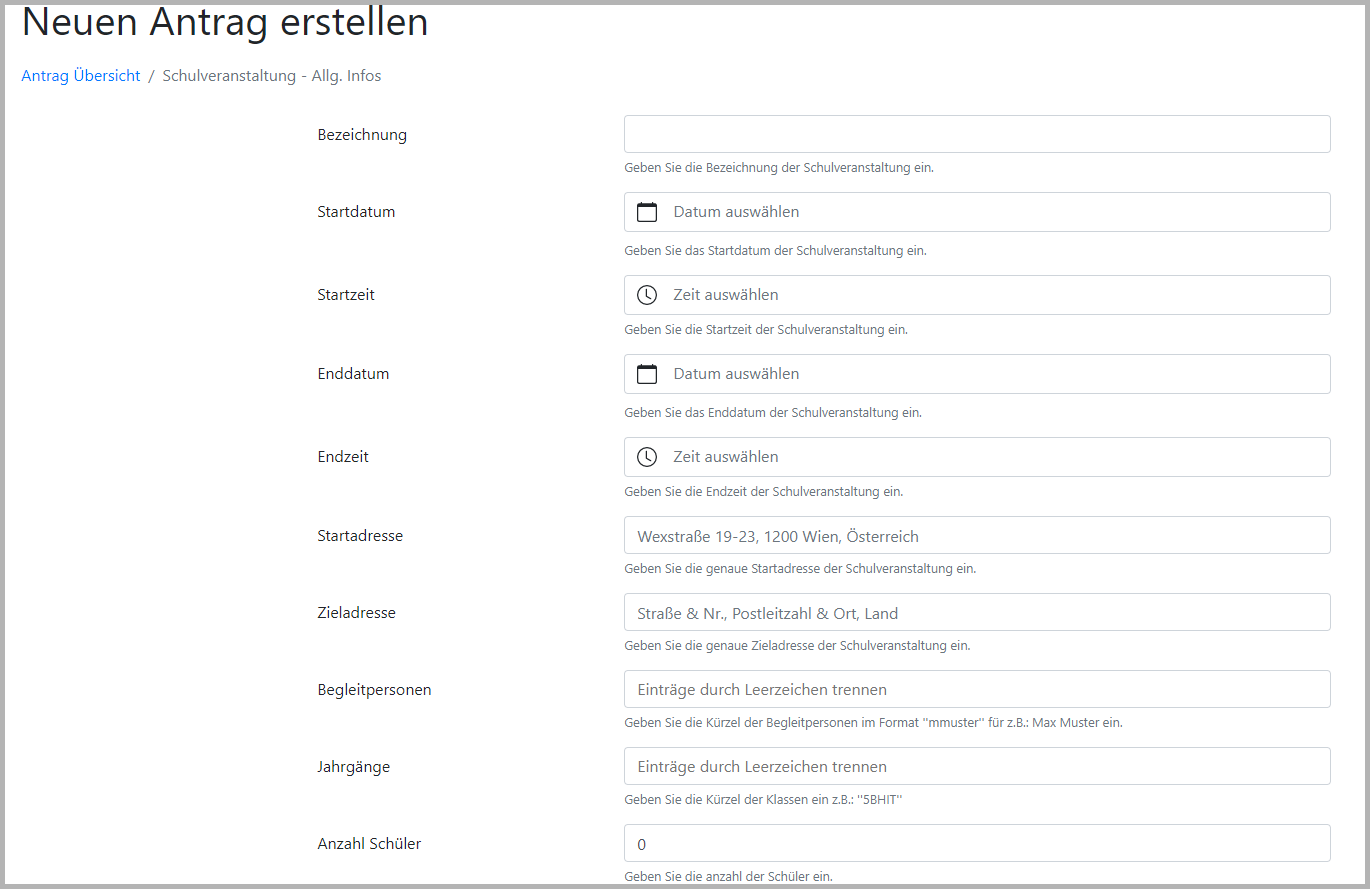
\includegraphics[width=1\linewidth]{images/website/schul_1}
	\caption[Neuer Schulantrag]{Ein Bild der Schulantrags Seite (Teil 1)}
	\label{fig:schulantrag1}
\end{figure}
\begin{figure}[H]
	\centering
	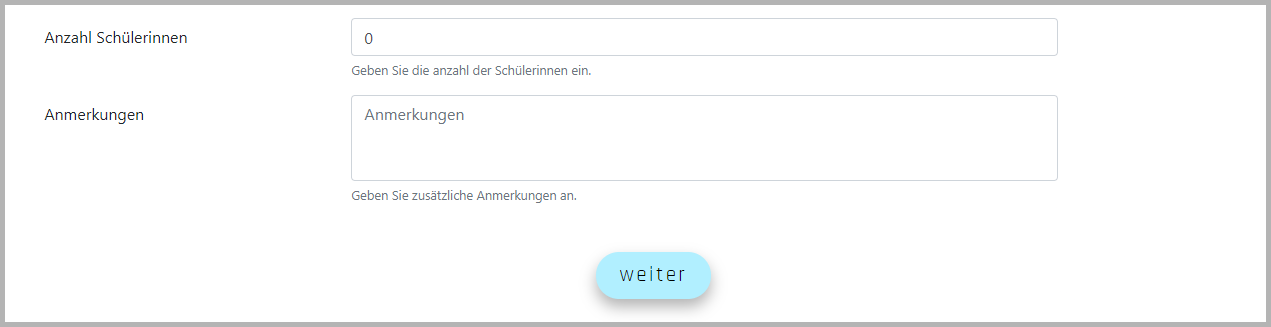
\includegraphics[width=1\linewidth]{images/website/schul_2}
	\caption[Neuer Schulantrag]{Ein Bild der Schulantrags Seite (Teil 2)}
	\label{fig:schulantrag2}
\end{figure}
Alle Eingabefelder sind in sogenannte \enquote{b-form-groups} eingefügt. Diese Elemente bieten die Möglichkeit, einen Titel, der in unserem Fall auf der linken Seite angebracht ist und eine Beschreibung, die unterhalb des Eingabefelds eingefügt ist hinzuzufügen - natürlich sind diese Elemente auch responsiv. In der \enquote{form-group} wird dann das jeweilige Element eingefügt, welches man eigentlich einbauen will. Diese Elemente können Beispielsweise normale Eingabefelder sein, Checkboxe, Radiobuttons, Timepicker, Datepicker, etc.. 
\begin{code}{html}
	<b-form-group
        id="bez"
        label-cols-sm="4"
        label-cols-lg="3"
        content-cols-sm
        content-cols-lg="7"
        description="Geben Sie die Bezeichnung der Schulveranstaltung ein."
        label="Bezeichnung"
        label-for="bezeichnung"
    >
        <b-form-input
            id="bezeichnung"
            v-model="data.Name"
            :readonly="readonly"
            @input="updateData"
        ></b-form-input>
    </b-form-group>
\end{code}
\captionof{listing}{Beispiel für eine Eingabegruppe}
Das Timepicker Element kann ganz einfach, wie im oberen Absatz beschrieben, in eine Eingabegruppe eingefügt werden. Da das Element von Bootstrap vordefiniert ist, muss man leidiglich die üblichen Werte, wie ID und Platzhalter setzen. Das Einzige was man wirklich beachten muss, ist, dass man die Richtige Zeitzone (Auflistung 7.13 locale) wählt.
\begin{code}{html}
	<b-form-timepicker
		id="stz"
		v-model="startTime"
		:readonly="readonly"
		@input="updateTime"
		locale="de"
		placeholder="Zeit auswählen"
  	></b-form-timepicker>
\end{code}
\captionof{listing}{Timepicker}
Der Datepicker ist noch einfacher zu bedienen, als der Timepicker. Hier sind nur die üblichen Parameter zu setzen.
\begin{code}{html}
	<b-form-datepicker
		id="end"
		v-model="endDate"
		:readonly="readonly"
		@input="updateTime"
		class="mb-2"
		placeholder="Datum auswählen"
  	></b-form-datepicker>
\end{code}
\captionof{listing}{Datepicker}
	\label{list:bspinputgroup} ~\\
Aus den im Formular angegebenen Daten, wird automatisch ein weiteres Formular generiert. Dies geschieht, nachdem der \enquote{weiter} Button betätigt wurde und alle Daten als Valide anerkannt wurden. Das Formular beinhaltet für jede Begleitperson die geforderten Eingabefelder (Abbildung 7.7). Die Struktur dieser Elemente ist exakt die Selbe, wie die, der Elemente, die in Abbildung 7.11 besprochen wurden. 
\begin{figure}[H]
	\centering
	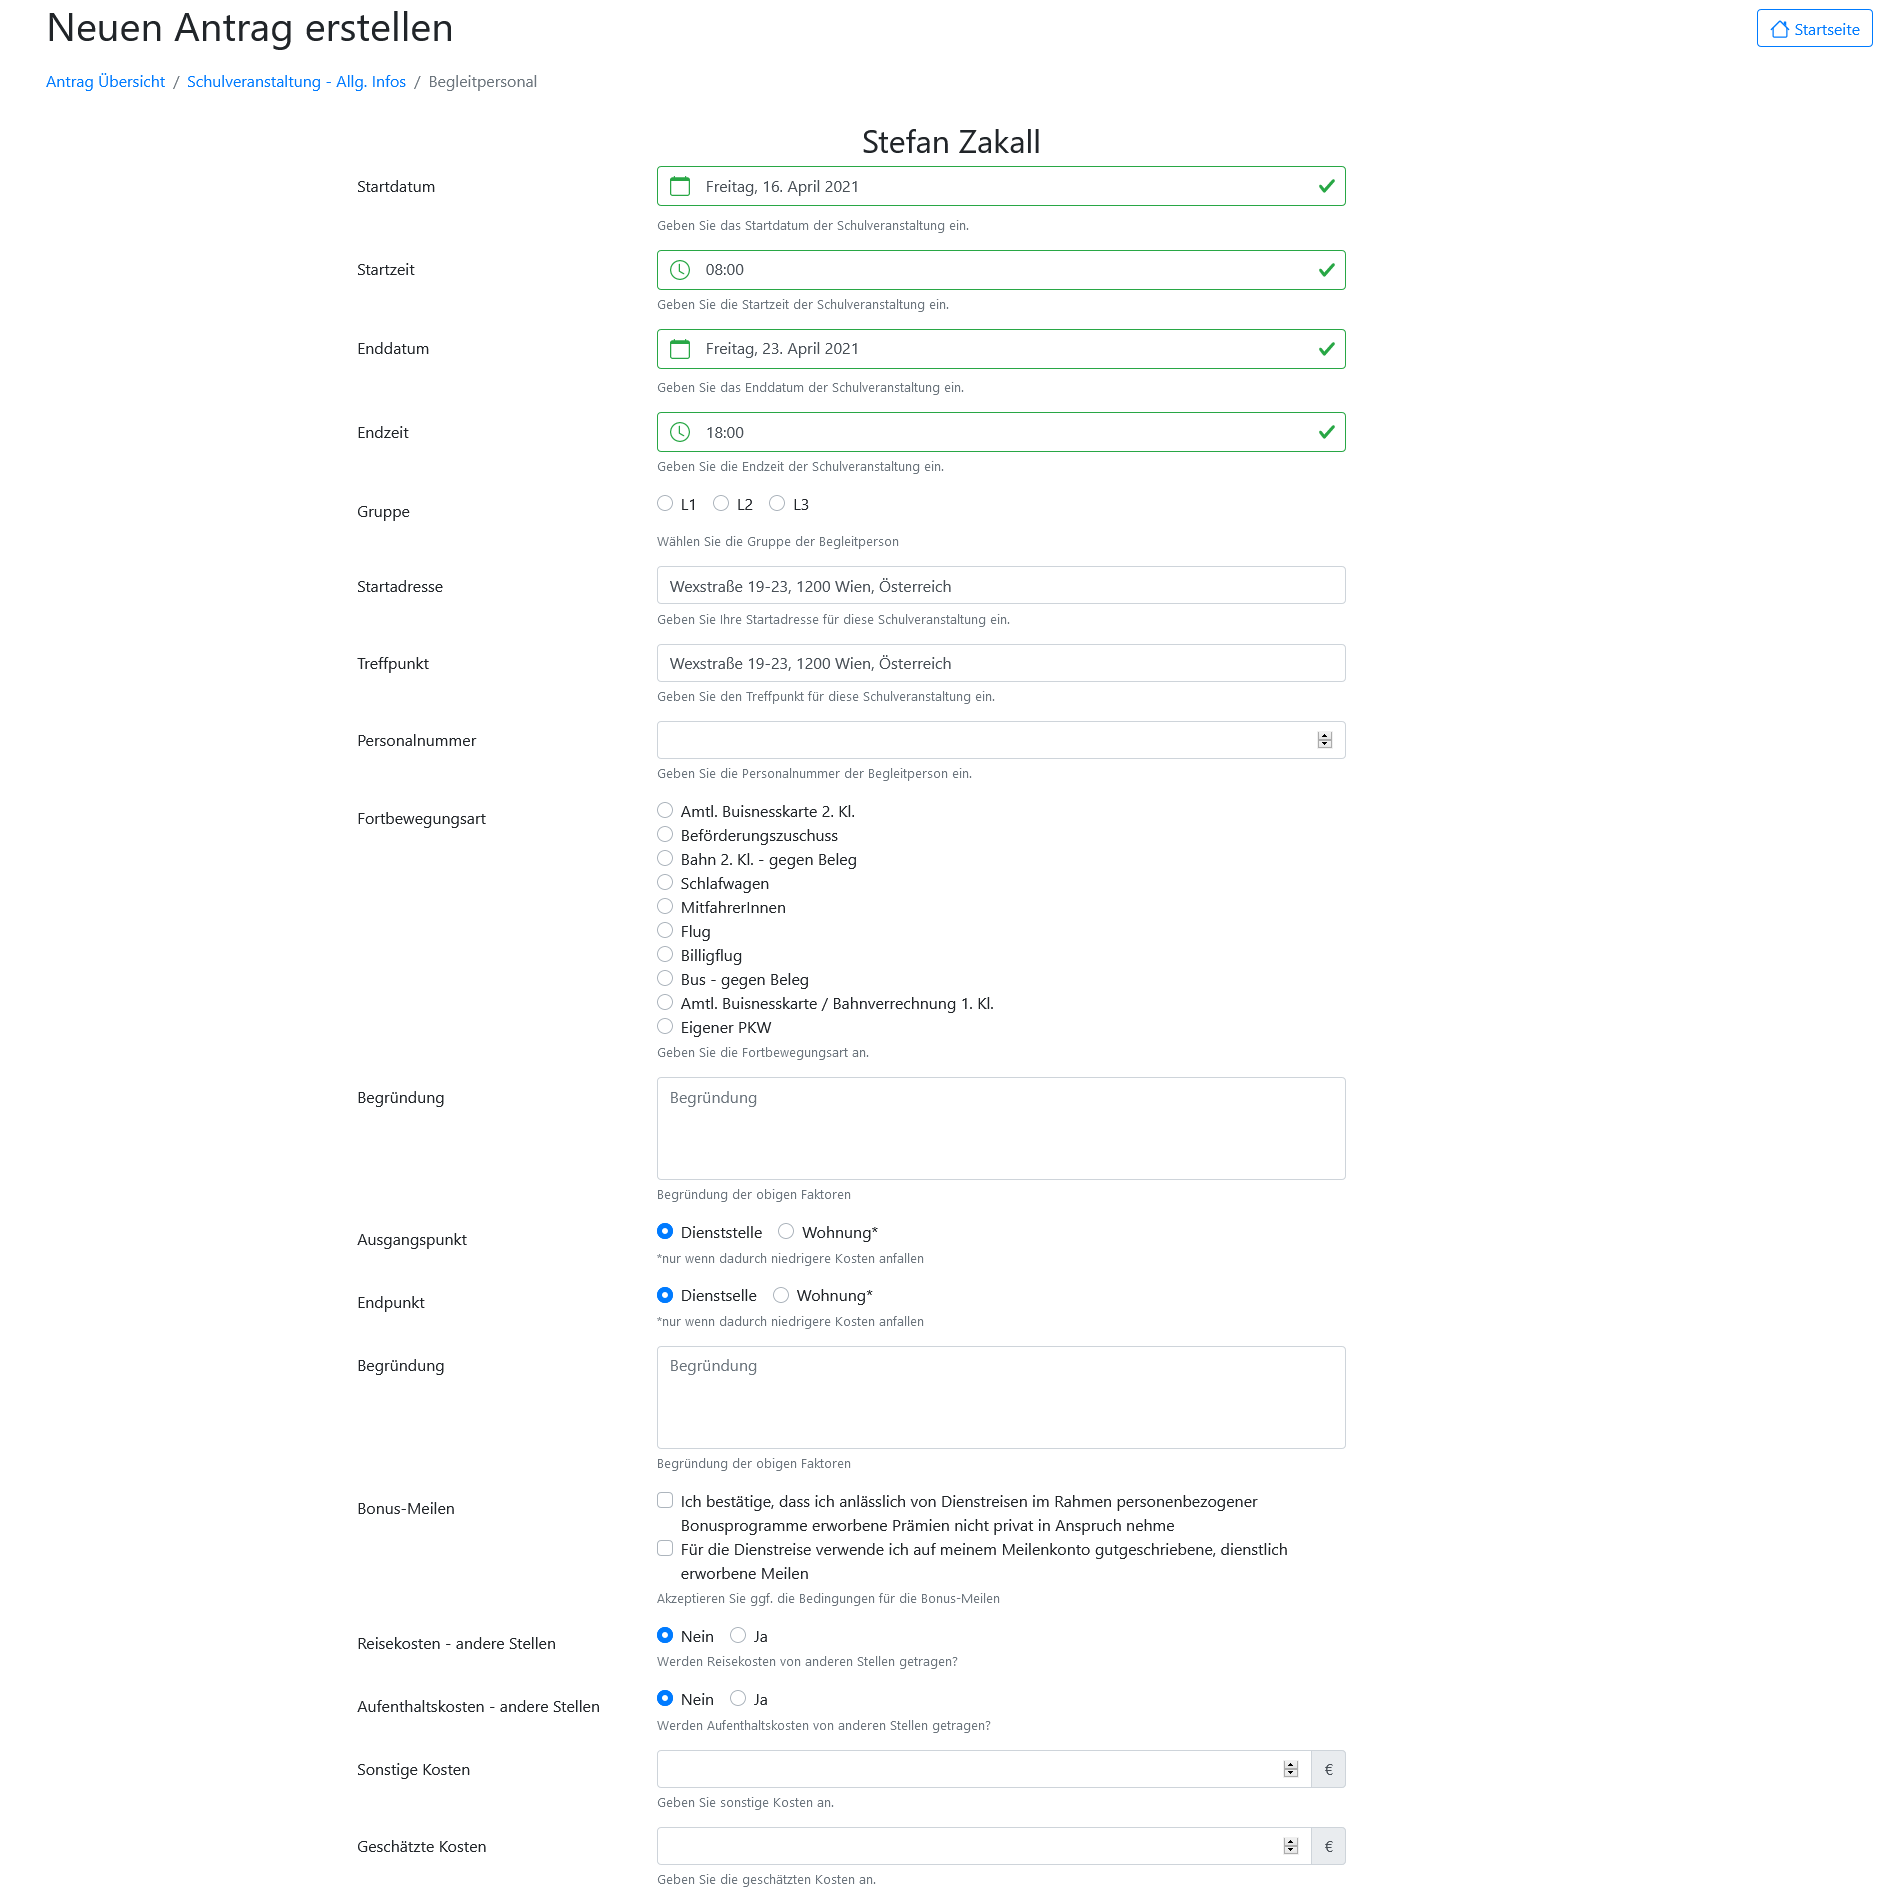
\includegraphics[width=1\linewidth]{images/website/schul_3_1}
	\caption[Neuer Schulantrag]{Ein Bild des Begleitformulars (Teil 1)}
	\label{fig:schulantrag3}
\end{figure}
\paragraph{Fortbildung}
Das Fotrbildungsformular ist für Seminare, Tagungen, Lehrgänge und sonstige Events in dieser Art gedacht. Um die Formulare einheitlich zu halten, wurde auch hier wieder die selbe Struktur der Eingabefelder verwendet. Falls man die sonstige Art auswählt, fügt sich automatisch eine zusätzliche Eingabe hinzu, in der man das Anliegen genauer spezifizieren kann.
\begin{figure}[H]
	\centering
	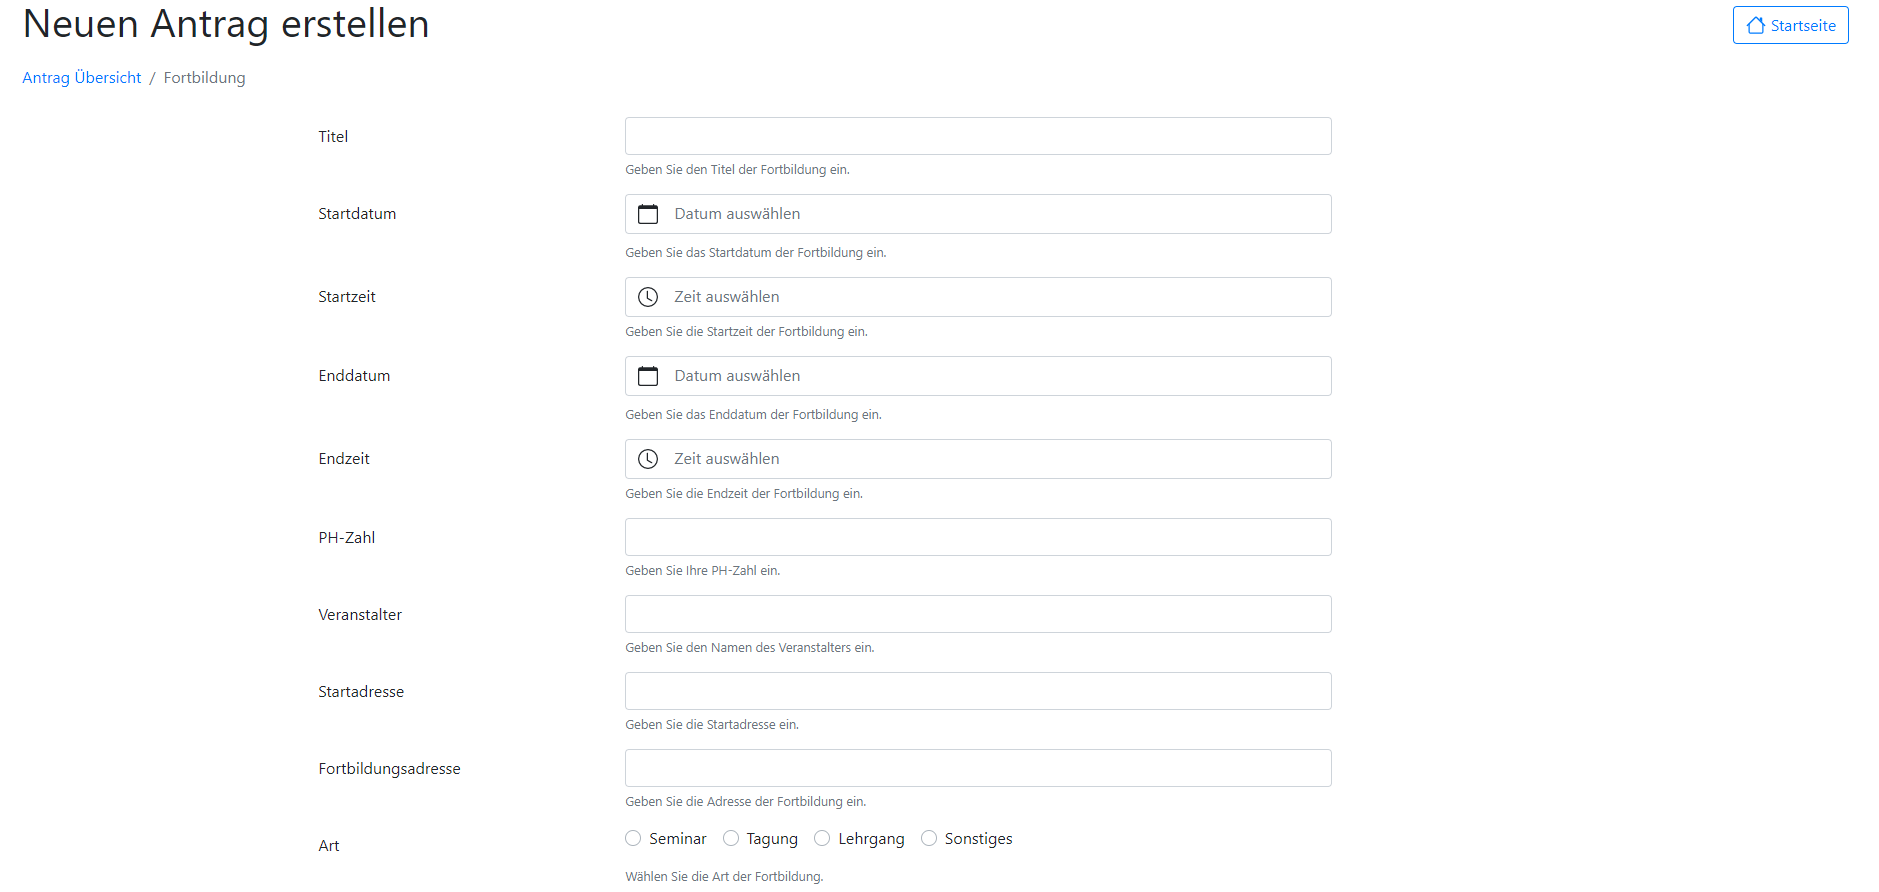
\includegraphics[width=1\linewidth]{images/website/fortbildung_1}
	\caption[Neuer Schulantrag]{Ein Bild des Begleitformulars (Teil 2)}
	\label{fig:frotbildung}
\end{figure}

\paragraph{Sonstige Anträge}
Zu den sonstigen Anträgen gehören Anliegen, wie Pflegefreistellungen, Dienstaufträge, Arzttermine und sonstige Freistellungen dieser Arten. Wählt man einen Dienstauftrag als Art aus erscheinen automatisch noch Eingabefelder, die das Eingeben der GZ und des Titels, des Dienstauftrages ermöglichen.
\begin{figure}[H]
	\centering
	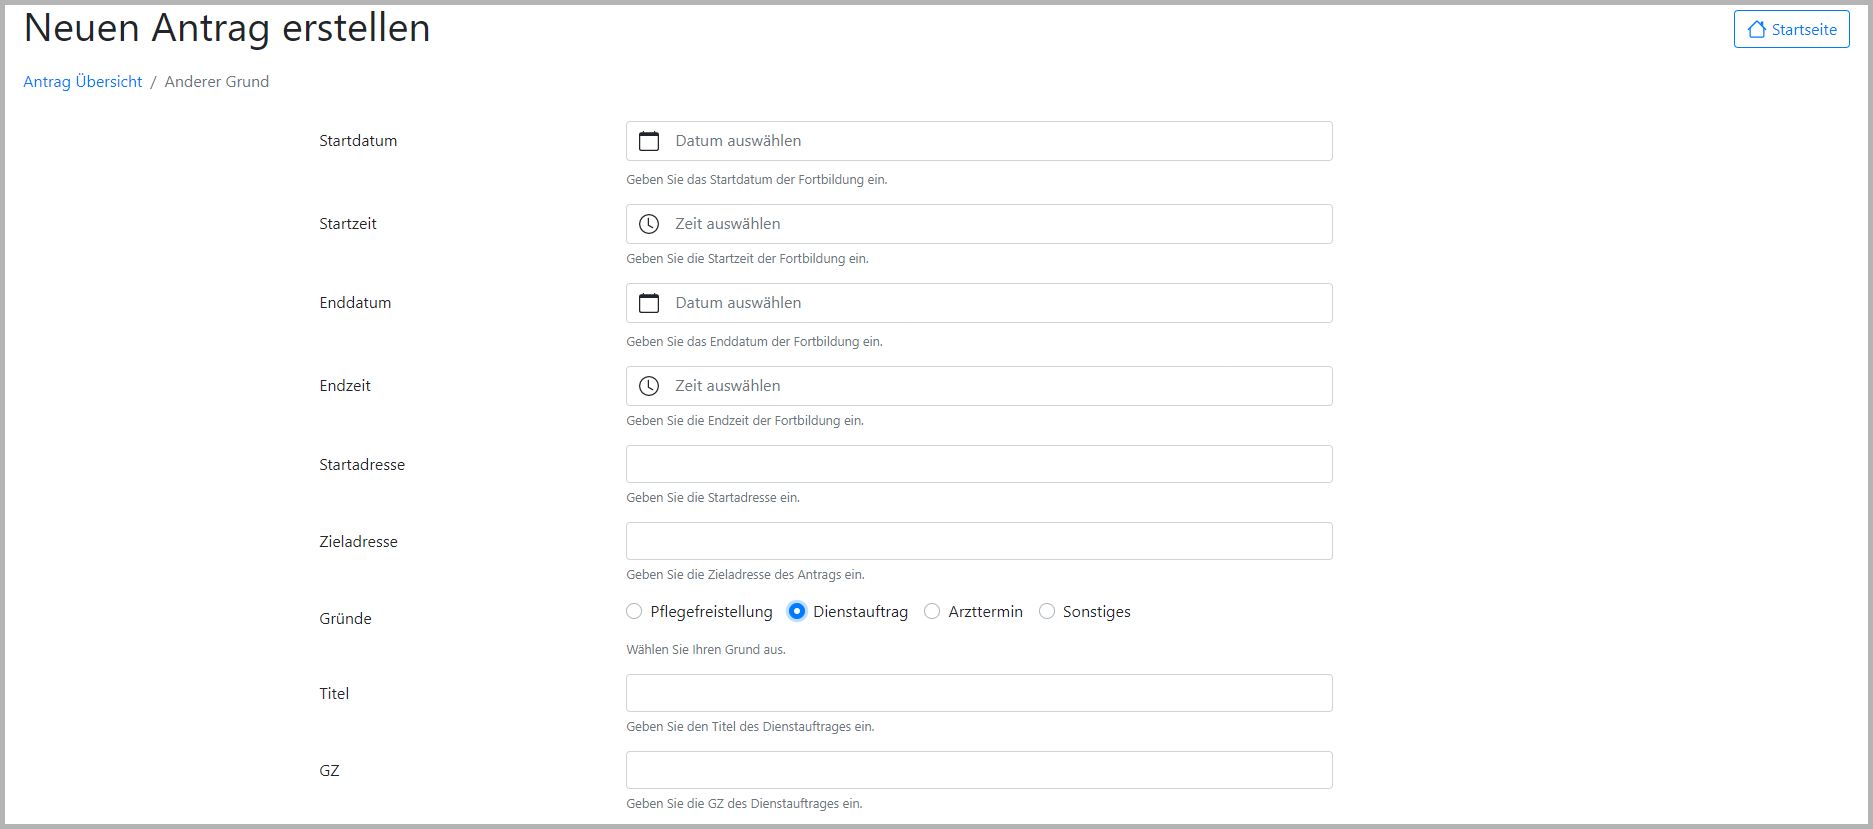
\includegraphics[width=1\linewidth]{images/website/dienstauftrag}
	\caption[Neuer Schulantrag]{Ein Bild des Begleitformulars (Teil 2)}
	\label{fig:dienst}
\end{figure}

\paragraph{Reiseantrag}
Der Reiseantrag wird automatisch bei den Formularen, der Anträge angehangen, bei denen eine Reise nötig ist. Ist keine Reise für einen bestimmten Antrag (zum Beispiel ein Arztbesuch) vorgesehen, dann wird das Formular nicht angehangen und es müssen keine unnötigen Daten eingegeben werden. Die Struktur der Elemente ist ident zu denen, die bereits besprochen wurden.
\begin{figure}[H]
	\centering
	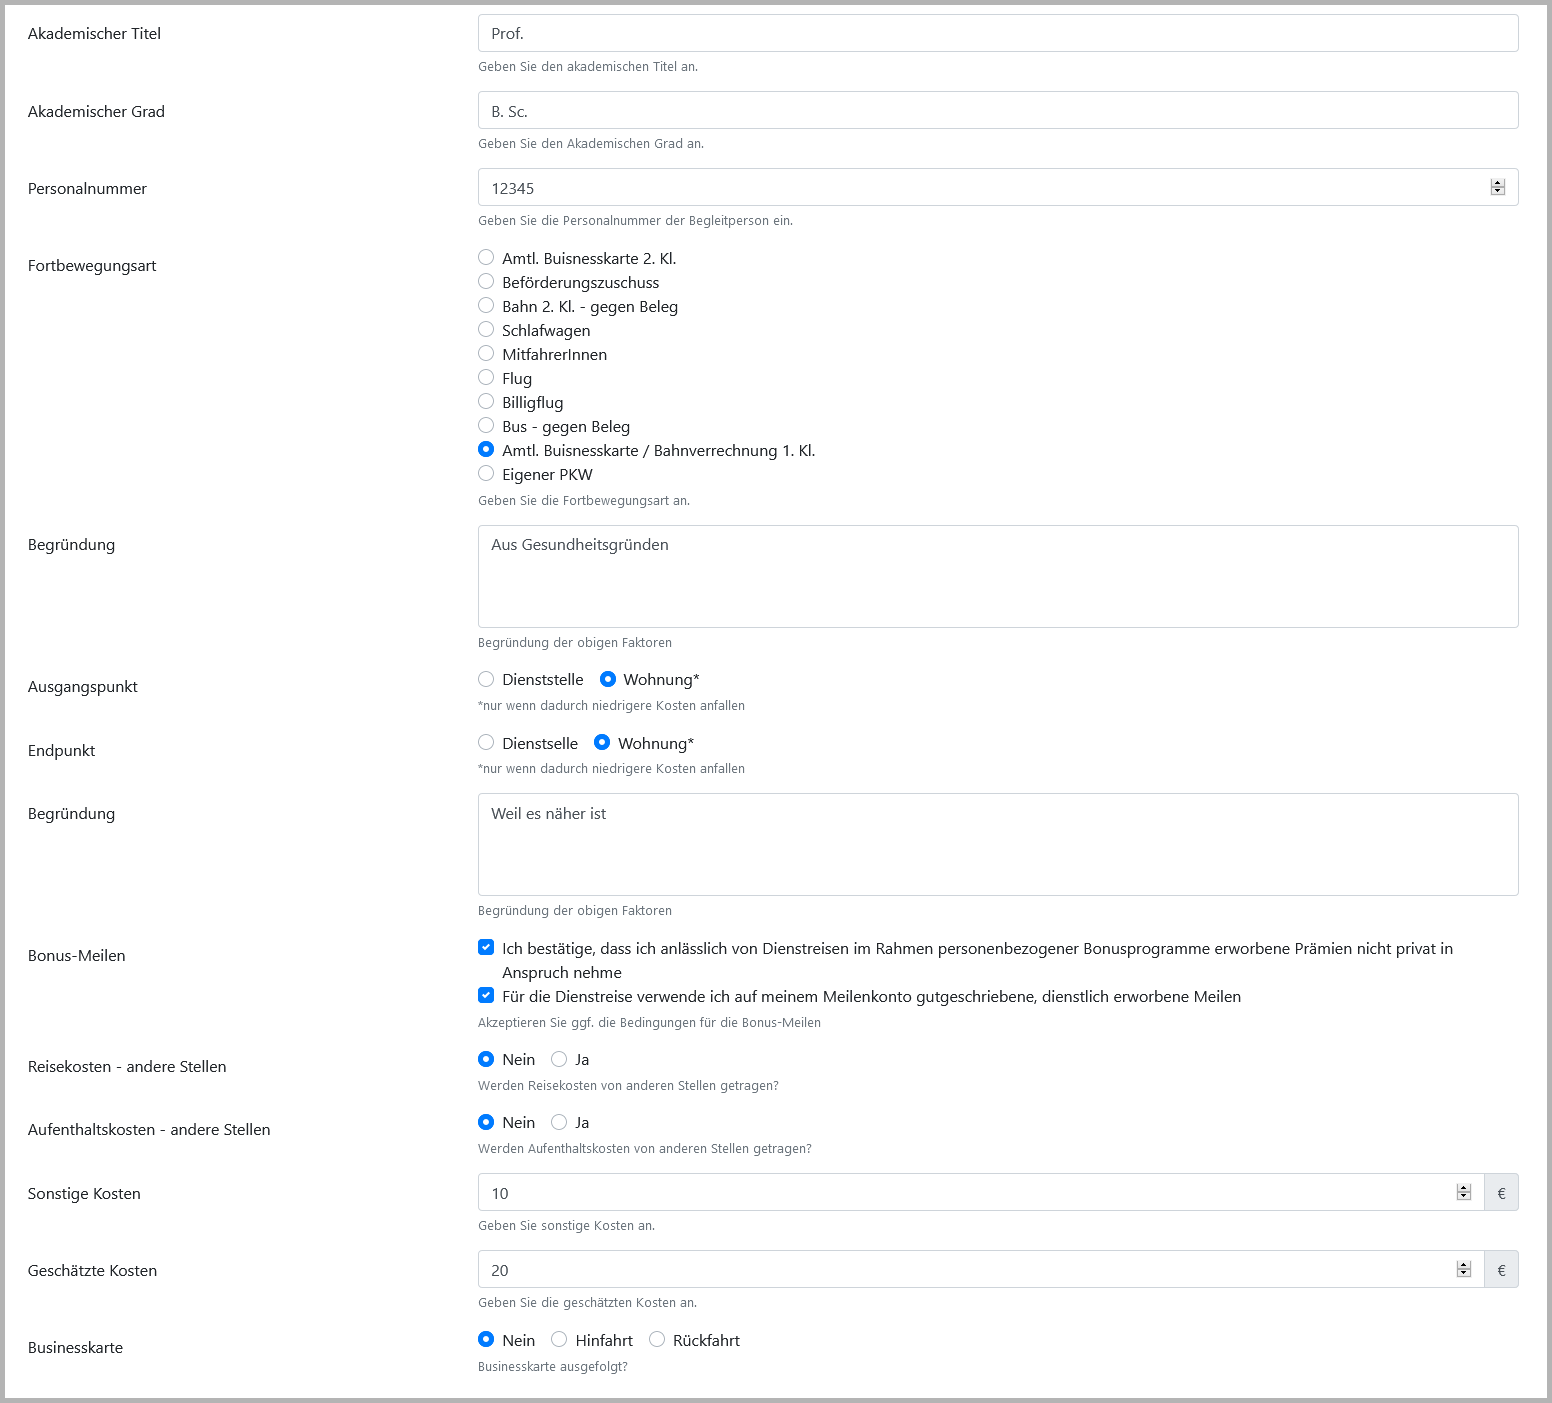
\includegraphics[width=1\linewidth]{images/website/zusatz_1.png}
	\caption[Neuer Schulantrag]{Ein Bild des Reiseantrages (Teil 2)}
	\label{fig:zusatz1}
\end{figure}
\begin{figure}[H]
	\centering
	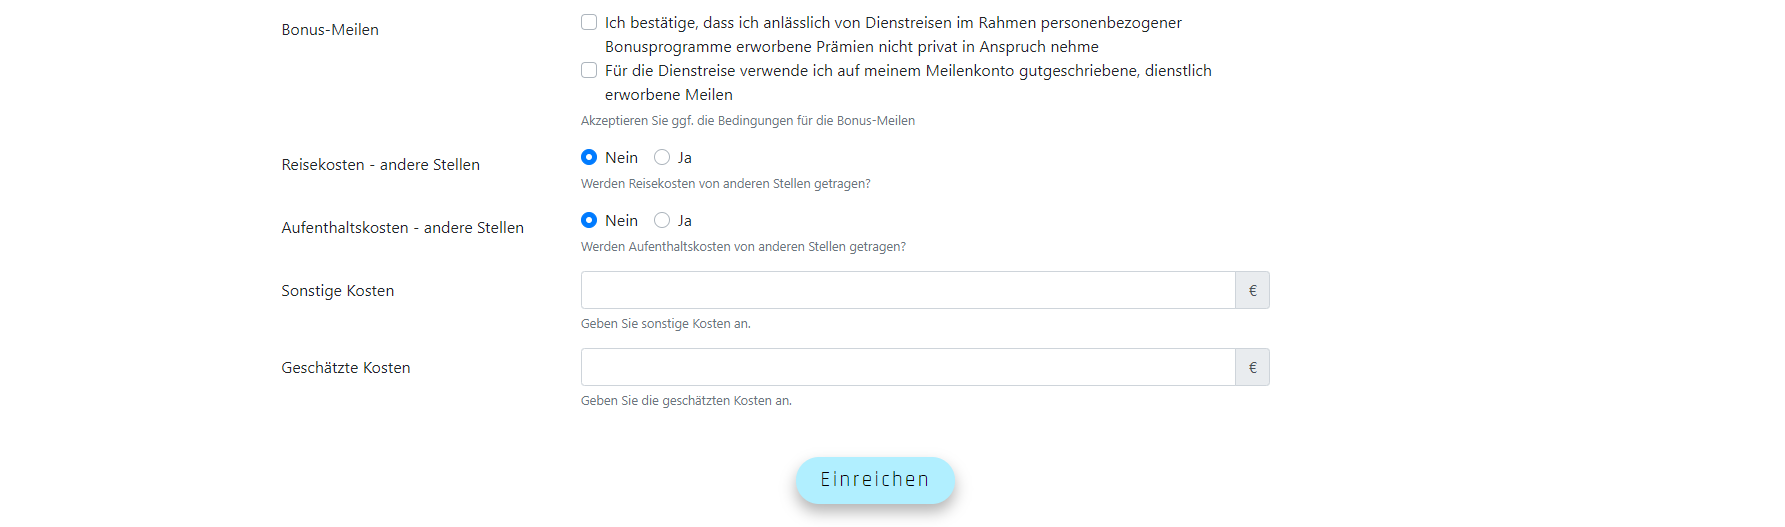
\includegraphics[width=1\linewidth]{images/website/zusatz_2.png}
	\caption[Neuer Schulantrag]{Ein Bild des Reiseantrages (Teil 2)}
	\label{fig:zusatz2}
\end{figure}

\newpage
\subsubsection{Ansicht Alle Anträge}
~\\

\newpage
\subsubsection{Ansicht Aktive Anträge}
~\\

\newpage
\subsubsection{Antragsansicht}
~\\
\paragraph{Fortschrittsanzeige}
~\\
\paragraph{Dokumente anzeigen}
~\\
\paragraph{Reiserechnung ausfüllen}
~\\
\paragraph{Funktionen}
~\\

\newpage
\subsubsection{Administrator Ansicht}
~\\

\newpage
\paragraph{Administrator Antragsansicht}
~\\

\newpage
\subsubsection{Seite nicht Gefunden}
~\\

\newpage
\subsubsection{Antrag suchen}
~\\

\newpage
\subsubsection{Rechte vergeben}
~\\


